% Section 8: The Policy index and the Strategic Index.
% Specification: R/categories/policy/{iea_policy_index,cat_policy_index}.R,
% R/indices/build_policy_index.R (build_composite_policy_index; POLICY_COMPONENT_WEIGHTS = IEA PAMS 3,
% CAT 2; IEA PAMS required), R/indices/build_indices.R (build_strategic_index,
% strategic_index_degenerate_sectors, strategic_index_es_floor_sectors, strategic_resource_base,
% flag_strategic_resource_base, select_allied_strategic_sectors), the policy block of
% scripts/10_build_themes.R and scripts/20_build_indices.R. Numbers: paper/results/strategic.json and
% si_fixed_inputs.json (final rerun of 2026-10-12); figures and table: scripts/paper/fig_strategic.R,
% fig_si_fixed_inputs.R. POL^*_{its} is the within-country S-curve of the Policy index (the code's pol).
% Further detail: sections/oa_strategic.tex (oa:strategic).
\section{The Policy index and the Strategic Index}\label{sec:strategic}

This section constructs a Policy index $\POL_{its}$ of recorded policy activity in each cell and a
Strategic Index $\SI_{its}$ that combines it with the two pillars and two fixed sector weights into
a ranking of each country's sectors, from which one allied pick is drawn for each coalition member.
Both have normative weights \citep{oecd2008handbook,decancq2013weights}; we state each and report
the choices to which the rankings are sensitive.

\subsection{The Policy index}\label{subsec:policy_composite}

No measure of industrial policy captures whether a policy is well designed
\citep{juhasz2024new,juhasz2022who,evenett2024return}. The Policy index measures the intensity and
direction of state attention to a cell, which indicates where capacity is likely to be built and
sustained \citep{rodrik2004industrial,rodrik2014green}, not whether that attention is warranted. It
has two components.

\paragraph{IEA Policies and Measures.}\label{subsec:policy_iea} The IEA database records national,
subnational and international energy and climate policies with their status, jurisdiction, type and
text \citep{iea2026pams}. Each policy $h$ is assigned to technologies and stages by keyword rules and
given a strength $\sigma_h$, the product of type, status and jurisdiction weights and of discounts
for cross-cutting or text-only assignments. The component is the S-curve of the log summed strength,
ranked over all country--technology--stage cells jointly so that it keeps differences in policy
density across countries and sectors,
\begin{equation}\label{eq:iea_index}
  x^{\mathrm{IEA}}_{its}={\Scurve}\Big[\log\Big(1+\textstyle\sum_{h\in\mathcal{H}_{its}}\sigma_h\Big)
  \Big]_{\mathrm{all}}.
\end{equation}
Online Appendix~\ref{oa:strategic} gives the tagging rules and weights.

\paragraph{Climate Action Tracker.}\label{subsec:policy_cat} The CAT component interacts a country's
overall climate-policy rating, mapped to $\kappa_i\in\{0.25,0.5,0.75,1\}$ (critically insufficient
to almost sufficient; \citealp{cat2026ratings}), with the technology weight $g_t$ defined below,
\begin{equation}\label{eq:cat}
  x^{\mathrm{CAT}}_{its}=\kappa_i\,g_t+(1-\kappa_i)(1-g_t)\qquad\text{for every stage } s.
\end{equation}
Its slope in $g_t$ is $2\kappa_i-1$: a rating of ``insufficient'' or better tilts a country's cells
toward clean technologies, ``highly insufficient'' leaves them flat and ``critically insufficient''
tilts them toward fossil ones (Figure~\ref{fig:si_fixed_inputs}, panel a). EU members without a
rating of their own take the EU's.

\paragraph{Composite and eligibility.} The Policy index is the weighted mean of the components
observed in the cell,
\begin{equation}\label{eq:pol_composite}
  \POL_{its}=\frac{\sum_{v\in\mathcal{V}_{its}}\omega_v\,x^{v}_{its}}
                  {\sum_{v\in\mathcal{V}_{its}}\omega_v},\qquad
  (\omega_{\mathrm{IEA}},\omega_{\mathrm{CAT}})=(3,2).
\end{equation}
The IEA component is required and CAT is added where the Tracker rates the country. All 215
economies in the IEA database receive an index: 65 on both components and 150 on the IEA component
alone, with the basis recorded. Requiring both components, the rule until October 2026, is a
robustness variant.

\paragraph{Why NIPO and the dual-use score are excluded.}\label{subsec:policy_nipo} Earlier versions
of the composite also carried the New Industrial Policy Observatory of Global Trade Alert
\citep[NIPO;][]{gta2026nipo,evenett2024return}, with weight 4, and a dual-use score, with weight 1.
The dual-use score is a project-authored judgement of each sector's defence relevance, identical
for every country: it measures no country and would act as a further sector prior read as policy.
NIPO is the most direct measure of industrial policy, but its allocation through product codes
reaches only Upstream and Midstream cells, which changed the effective weights by stage, and the
component available when the composite was fixed covered 23 economies. It returns as a robustness
variant built from the October 2026 run (77 jurisdictions; Online Appendix~\ref{oa:strategic}).

\subsection{The Strategic Index}\label{subsec:si_definition}

For a cell in the sample, the index is
\begin{equation}\label{eq:si}
  \SI_{its}=0.2\,\POL^{*}_{its}+0.3\,\EO_{its}+0.3\,(1-\ES_{its})+0.1\,\lambda_s+0.1\,g_t,
\end{equation}
where the policy term is the within-country S-curve of the Policy index over the country's
in-sample sectors,
\begin{equation}\label{eq:si_pol}
  \POL^{*}_{its}={\Scurve}\big[\POL\big]_{i}\qquad\text{over }
  \big\{(t',s'):\ (i,t',s')\ \text{in the sample}\big\},
\end{equation}
and $\EO_{its}$ and $\ES_{its}$ enter at their cross-country levels. Every term lies in $[0,1]$ and
the weighted terms add up to the index exactly.

\paragraph{Policy, need and scaling.} The policy term rewards the sectors on which a government
already concentrates its attention, where programmes and administrative capacity make further
effort more likely to succeed \citep{rodrik2004industrial,juhasz2024new}. It is ranked within the
country because the volume of recorded policy depends on governments' transparency and compilers'
attention; the pillars keep their cross-country levels, so that a sector in which a country leads
the world counts for more than one in which it is merely its own best. Security enters as need,
$1-\ES_{its}$: new capacity is most valuable where it reduces an exposure rather than duplicating a
strength (Section~\ref{sec:framework}); the strength reading is reported below. Nominal weights are
not effective weights \citep{paruolo2013ratings,becker2017weights}, and the index ranks sectors
within a country rather than comparing levels across countries.

\paragraph{Fixed sector weights.} The stage weights are $\lambda_{\mathrm{Midstream}}=0.75$,
$\lambda_{\mathrm{Upstream}}=0.5$ and $\lambda_{\mathrm{Downstream}}=0.25$: clean-energy supply chains
are most concentrated in processing and manufacturing \citep{iea2021role,iea2024etp}, extraction is
bound to geology and deployment is largely non-traded. The technology weight $g_t$ is a min-max index of
lifecycle greenhouse-gas intensity. With $c_r$ the median intensity (gCO$_2$e/kWh) of generation
technology $r$ and $R_t$ the rows of technology $t$,
\begin{equation}\label{eq:ghg_index}
  g_t=\frac{1}{|R_t|}\sum_{r\in R_t}\frac{\max_{r'}c_{r'}-c_r}{\max_{r'}c_{r'}-\min_{r'}c_{r'}}\in[0,1],
\end{equation}
from the AR5 lifecycle medians \citep{schlomer2014annex} and, for oil-fired generation, the SRREN
median of 840 gCO$_2$e/kWh \citep{moomaw2011annex}; technologies without a row take proxies (Online
Appendix~\ref{oa:strategic}). The weight runs from 0 for oil, 0.02 for coal and 0.42 for gas to 0.97
for solar and 0.999 for nuclear and wind. The two weights add a sector prior of 0.025 (Oil
Downstream) to 0.175 (Wind Midstream) to every country's index (Figure~\ref{fig:si_fixed_inputs},
panel b): a stated preference for clean, midstream activity, not a measurement, which decides the
ranking where a country's measured terms are flat. The same $g_t$ scales the climate penalty of the
bilateral indices (Section~\ref{sec:bilateral}).

\paragraph{Implicit sector priors.} Because the pillars enter at their cross-country levels, two
further sector-level terms act as priors in each country's ranking, in addition to the stage and
technology weights. Inputs that are the same for every economy in a pair (world demand, market size
and overcapacity, TRL, price volatility and the world-concentration terms of Trade) shift that
pair's pillar levels for all countries; on the scored cells they contribute on average 0.18 to
$\EO_{its}$ and 0.07 to $\ES_{its}$, and their net contribution to the index varies across sectors
from $-0.065$ to $0.012$. And stage-level differences in zero-inflation (in the median Upstream pair
71 percent of rankable economies score zero on Reserves; Section~\ref{sec:es}) lower Upstream
security and so raise Upstream need for every country. The first term can be measured: across the
57 allied picks, the cell-constant inputs account for a median of 45 percent of the margin over
the runner-up, favour the pick in 36 cases and exceed the whole margin in 18. Removing them from the
pillar levels keeps 29 of the 57 picks, and entering opportunity and need as within-pair ranks keeps
27 (Section~\ref{sec:robustness}).

\begin{figure}[tbp]
  \centering
  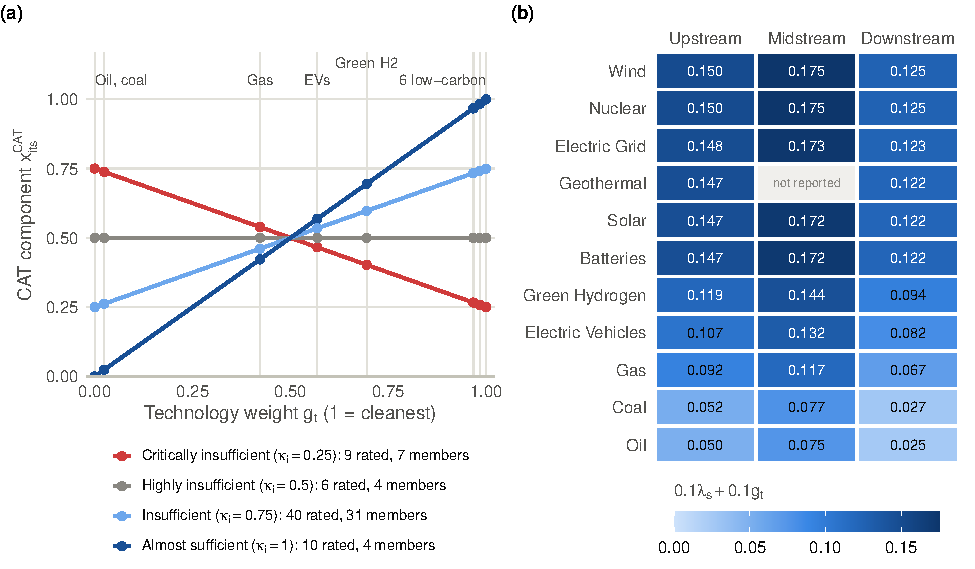
\includegraphics[width=\textwidth]{fig_si_fixed_inputs}
  \caption{The country-invariant inputs of the Strategic Index. Panel (a): the Climate Action
  Tracker component of the Policy index, $x^{\mathrm{CAT}}_{its}=\kappa_ig_t+(1-\kappa_i)(1-g_t)$,
  against the technology weight $g_t$ (IPCC life-cycle emissions, 1 = cleanest) for the four CAT
  ratings, with the eleven technologies marked on each line; the slope is $2\kappa_i-1$. The legend
  counts the countries CAT rates in each category in the final build (65 in all, 26 of them EU
  members through the EU's rating) and the coalition members among them (46 of 57: 31
  insufficient, 7 critically insufficient, 4 highly insufficient, 4 almost sufficient). Panel (b):
  the sector prior $0.1\lambda_s+0.1g_t$ that the stage weights $\lambda_s$ (Upstream 0.5, Midstream
  0.75, Downstream 0.25) and the technology weights add to the Strategic Index of every country;
  Geothermal Midstream is not a reported sector. Source: the pipeline's functions and
  \texttt{data/raw/ipcc\_ghg\_intensity.csv}, with the CAT ratings of \texttt{policy\_component\_tbl}
  in \texttt{index\_outputs.rds}; \texttt{scripts/paper/fig\_si\_fixed\_inputs.R}.}
  \label{fig:si_fixed_inputs}
\end{figure}

\subsection{Sample rules and the allied pick}\label{subsec:si_sample}

Nothing is imputed in the Strategic Index. A cell is scored only if the country has a Policy index
and both of its pillar cells are rankable under the rule of Section~\ref{sec:normalization} (the
economy is sovereign and at most half of each pillar cell's index weight is imputed); an unscored
cell stays in the output with its reason recorded. Geothermal Midstream, which has no Energy
Security pillar, is excluded by rule; a check that removes any sector whose pillar is constant
across the scored countries finds none in the final build.

\paragraph{Allied pick.}\label{subsec:si_allied} For each coalition member $i$, let $\mathcal{A}_i$
be its scored Upstream and Midstream sectors outside Geothermal and Green Hydrogen, less the Upstream
sectors barred by the endowment screen below. The allied pick is
\begin{equation}\label{eq:si_allied}
  (t,s)^{\ast}_i=\argmax_{(t,s)\in\mathcal{A}_i}\ \SI_{its}.
\end{equation}
Only the traded stages, which coalition supply chains can organise across borders, are eligible;
Geothermal and Green Hydrogen have no HS6 basket and Midstream Energy Security pillars that are
constant or concentrated at one value. The pick summarises the index for each member, EU members
included; the network design does not use it.

\paragraph{Endowment screen.} With security read as need, an economy without a resource sits at the
floor of the extraction stage's Energy Security pillar and has maximal need there. The screen makes
an Upstream stage eligible for a member's pick only if the member has recorded reserves or
production of the stage's resources (technology-level Reserves or Production greater than zero). It
is a rule of the pick, not of the index: values are unchanged and screened cells are flagged.

\subsection{Results}\label{subsec:strategic_results}

\paragraph{Coverage and basis of the Policy index.} All 57 coalition members have a Policy index, 46
on both components and 11 on the IEA component alone: Israel and Ukraine in the core and nine
partners (the Democratic Republic of the Congo, the Dominican Republic, Gabon, Ghana, Guatemala,
Malaysia, Namibia, Oman and Qatar). The two components measure different things
(Figure~\ref{fig:strategic_policy}): over the 65 economies scored on both, their Spearman
correlation is $-0.05$ across cells and $-0.02$ within a country at the median, and the composite
follows the Tracker component within a country (median 0.79) more than the IEA one (0.48). Ranking
these countries' cells on the IEA component alone gives a median within-country Spearman of 0.48
with the composite over their policy cells and 0.44 over their Strategic Index cells: the basis
matters for a country's internal ranking.

\begin{figure}[tbp]
  \centering
  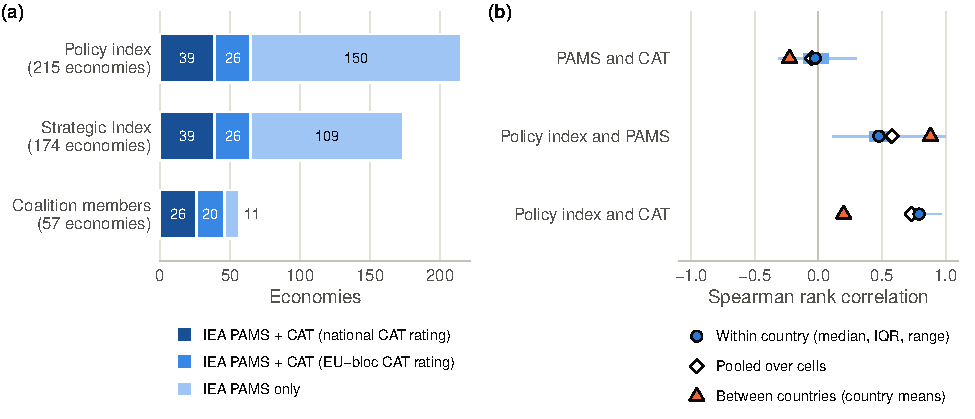
\includegraphics[width=\textwidth]{strategic_policy}
  \caption{The basis of the Policy index. Panel (a): number of economies by the components of their
  Policy index, for all economies with an index (215), the economies with a Strategic Index cell
  (174) and the coalition members (57). ``IEA PAMS + CAT'' combines the IEA Policies and Measures
  database (weight 3) with the Climate Action Tracker rating (weight 2), national or, for EU
  members, the Union's; ``IEA PAMS only'' marks economies the Tracker does not rate. Panel (b):
  Spearman correlations among the two components and the composite over the 33 cells of the 65
  economies scored on both: median, interquartile range and range of the within-country correlations
  (59 economies whose Tracker component varies across cells), pooled over cells and across country
  means. Source: \texttt{policy\_component\_tbl}, \texttt{policy\_index} in
  \texttt{index\_outputs.rds}.}
  \label{fig:strategic_policy}
\end{figure}

\paragraph{Sample and distribution.} The Strategic Index covers 3,154 cells of 174 countries in 30
sectors (Electric Grid Downstream and Geothermal Upstream have no scored cell). Of the 6,476 cells
of policy-eligible countries, 2,700 fail the rankability rule on one or both pillars and 622 lack an
Energy Security cell. Every coalition member is scored, with a median of 29 sectors. The index
(mean 0.535, standard deviation 0.082) is organised by sector far more than by country: sector fixed
effects explain 72.6 percent of its variance and country fixed effects 4.4 percent
(Figure~\ref{fig:strategic_heatmap}). The highest cells are Nuclear Upstream cells of small economies
without uranium, where Energy Security sits at a floor shared by 86 of the 174 countries and need is
maximal: Nuclear Upstream is the top sector of 62 countries, 55 of them without recorded uranium. This
construction effect of the need reading motivates the endowment screen. Green Hydrogen Midstream (34
of 40 countries at one value), Green Hydrogen Downstream, Nuclear Downstream and Batteries Downstream
also have floors; no allied pick lies in a floor cell.

\begin{figure}[tbp]
  \centering
  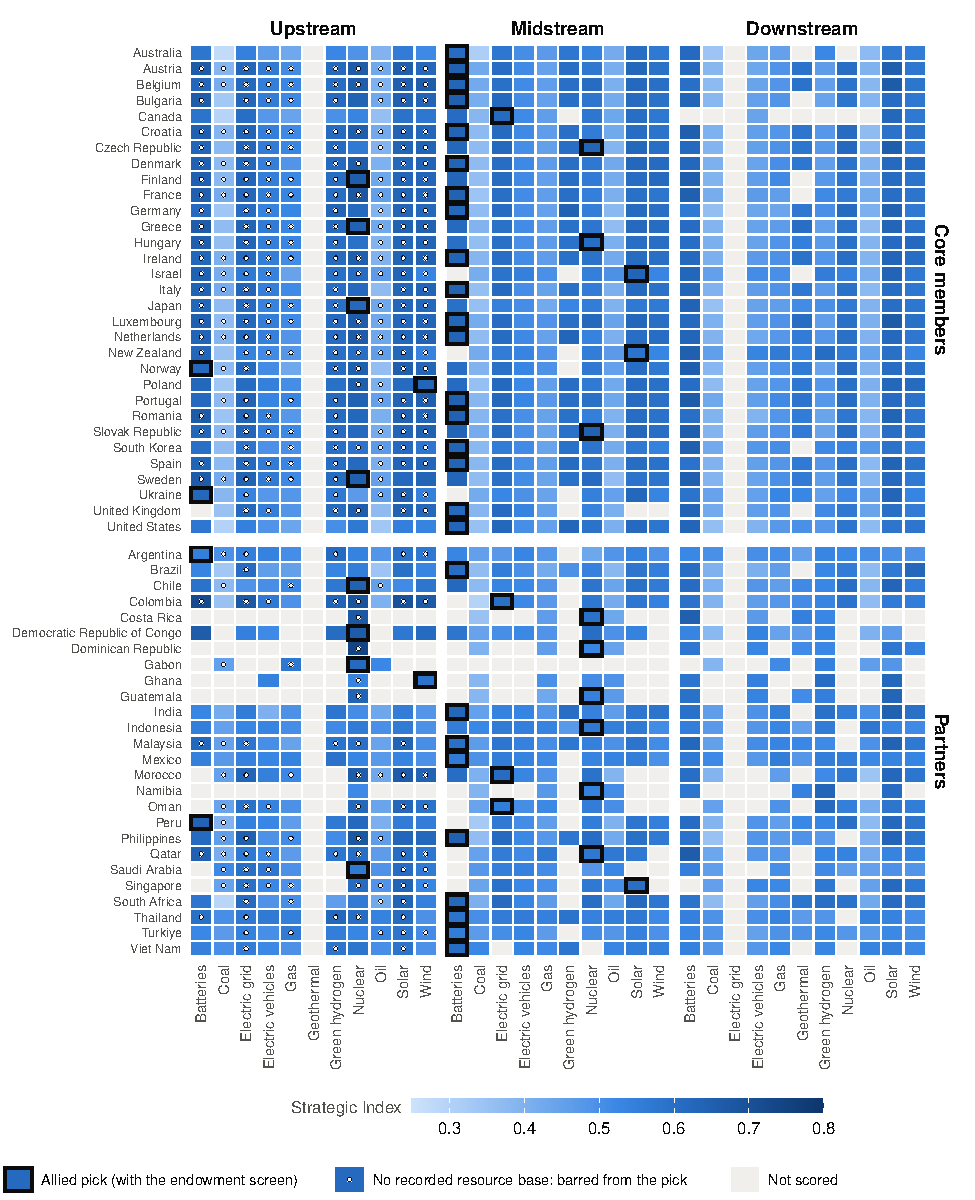
\includegraphics[width=0.94\textwidth]{strategic_heatmap}
  \caption{The Strategic Index across the coalition. Rows are the 57 members (31 core, then 26
  partners), columns the 33 technology--stage cells grouped by stage; colour is $\SI_{its}$
  (equation~\eqref{eq:si}). Grey cells are not scored (a pillar cell not rankable or missing, or
  Geothermal Midstream, excluded by rule). A dot marks an Upstream cell in which the member has no
  recorded reserves or production of the stage's resources: the endowment screen bars it from the
  pick, but its value is unchanged. The outlined cell in each row is the member's allied pick
  (equation~\eqref{eq:si_allied}). Source: \texttt{strategic\_index} in \texttt{index\_outputs.rds};
  \texttt{allied\_strategic.csv}.}
  \label{fig:strategic_heatmap}
\end{figure}

\paragraph{Decomposition.} The five terms account for 18.8 (policy), 27.6 (opportunity), 32.4
(need), 9.3 (stage) and 11.9 percent (technology) of the index level, but very different shares of
its within-country variance: on average 40.7 percent for the technology weight, 34.1 percent for
need and 32.0 percent for policy, against $-1.4$ percent for opportunity and $-5.4$ percent for the
stage weight. Opportunity moves against need (median within-country Spearman of $\EO$ and $1-\ES$
$-0.47$, negative in 164 of 167 countries; $-0.49$ and negative for all 57 coalition members), because a country's strongest opportunities tend to be
the sectors in which it is already secure; the two offset, and the ranking is set by the technology
weight, need and the policy rank (Figure~\ref{fig:strategic_decomp}).

\begin{figure}[tbp]
  \centering
  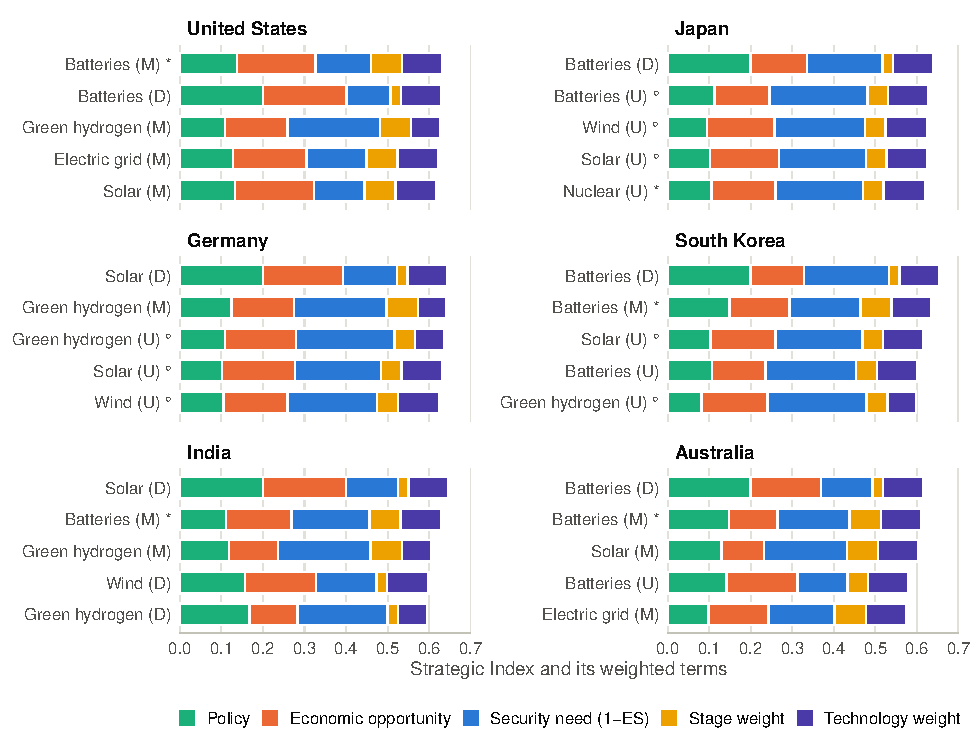
\includegraphics[width=\textwidth]{strategic_decomp}
  \caption{Decomposition of the Strategic Index for the five highest-ranked sectors of six coalition
  members. Each bar stacks the weighted terms of equation~\eqref{eq:si}: $0.2\,\POL^{*}_{its}$,
  $0.3\,\EO_{its}$, $0.3\,(1-\ES_{its})$, $0.1\,\lambda_s$ and $0.1\,g_t$; bar length is
  $\SI_{its}$. (U), (M) and (D) mark the stage; an asterisk marks the member's allied pick and a circle
  an Upstream sector barred by the endowment screen. Source: \texttt{strategic\_index} in
  \texttt{index\_outputs.rds}.}
  \label{fig:strategic_decomp}
\end{figure}

\paragraph{Allied picks.} Every member has a pick, and none is tied
(Table~\ref{tab:strategic_allied}). Batteries Midstream is the pick of 27 members (among them the
United States, Germany, Korea, India and Australia), Nuclear Midstream of nine, Nuclear Upstream of
eight, Batteries Upstream and Electric Grid Midstream of four
each, Solar Midstream of three and Wind Upstream of two (Ghana and Poland): 43 Midstream and 14
Upstream picks. The picks are sectors a member needs and supports with policy rather than sectors in
which it already competes: within a member's eligible sectors the pick ranks first on policy for 22
members and on need for 23, but on opportunity for none. The eight Nuclear Upstream picks (Chile,
the Democratic Republic of the Congo, Finland, Gabon, Greece, Japan, Saudi Arabia and Sweden) all
hold identified uranium resources, but small ones, 0.015 to 0.79 percent of world identified
resources below USD 260/kgU, and none has recorded mine production in 2019--2024. These picks are
still need-driven: a negligible resource ranks near the floor of the security pillar, so the
screen removes the no-resource artefact but not its small-resource counterpart. Requiring recorded
production rather than any reserves removes all eight Nuclear Upstream picks (seven members move
to another sector and Gabon is left without an eligible one) and the two Wind Upstream picks of
Ghana and Poland.

The picks are fragile. The median margin over the runner-up is 0.015; it is below 0.005 for 10
members (17.5 percent) and below 0.01 for 21 (36.8 percent), against a within-country standard
deviation of 0.080, so the table reports the runner-up beside each pick. The distribution also moved
during the final data revisions: in a run of 8 October, when 45 members had a pick, Electric Grid
Midstream was the pick of 17 and Batteries Midstream of 11, before completing the energy-trade file filled missing codes
of the grid basket.

The Nuclear Midstream picks of small partners are not an Energy Security floor effect. Costa Rica,
the Dominican Republic and Guatemala each have four eligible sectors, the Midstream stages of
nuclear, oil, gas and coal (Namibia these and Nuclear Upstream). The technology weight ($g_t=0.999$
for nuclear against 0.42 for gas, 0.02 for coal and 0 for oil) puts Nuclear Midstream's sector prior
0.058, 0.097 and 0.100 ahead of the three fuels, more than any other term separates pick from
runner-up, while Nuclear Midstream Energy Security is compressed around its median (interquartile
range 0.095, against 0.12--0.15 in the fossil Midstream sectors), so need adds only 0.020--0.042.

\paragraph{Picks and the network design.} The pick is a national priority read from need and
policy, not an allied assignment. Aggregated, the picks reproduce the duplication that an Allied
Industrial Base is meant to avoid: 27 members would prioritise Batteries Midstream, which the
network design of Section~\ref{sec:network} gives to nine producer nodes. Of the 27, 20 hold a
designed role in that stage, 14 of them only through the EU node, and seven (Australia, Brazil,
Mexico, the Philippines, South Africa, T\"urkiye and Viet Nam) do not. Across all members, 28 of
the 57 hold a designed share in their pick stage (the column ``Design share'' of
Table~\ref{tab:strategic_allied}), and eight (Costa Rica, the Dominican Republic, Gabon, Ghana,
Guatemala, New Zealand, T\"urkiye and Ukraine) produce nothing in the design.

% Generated by scripts/paper/fig_strategic.R -- do not edit by hand.
\begingroup
\singlespacing\scriptsize
\setlength{\tabcolsep}{2.9pt}
\setlength{\LTcapwidth}{\textwidth}
\begin{longtable}{@{}l l S[table-format=1.3] l S[table-format=1.4] c l c c@{}}
\caption{Allied strategic selection: pick, runner-up, margin and robustness of the pick}
\label{tab:strategic_allied}\\
\toprule
 & & & & & & & \multicolumn{2}{c@{}}{\makecell{Same pick\\under}}\\
\cmidrule(l){8-9}
Member & Pick & {$\SI$} & Runner-up & {Margin} & \makecell{AIB\\coalitions} & \makecell[l]{Pick without\\the screen} & (1) & (2)\\
\midrule
\endfirsthead
\multicolumn{9}{@{}l}{\small\textbf{Table \thetable:} continued}\\
\toprule
 & & & & & & & \multicolumn{2}{c@{}}{\makecell{Same pick\\under}}\\
\cmidrule(l){8-9}
Member & Pick & {$\SI$} & Runner-up & {Margin} & \makecell{AIB\\coalitions} & \makecell[l]{Pick without\\the screen} & (1) & (2)\\
\midrule
\endhead
\midrule
\multicolumn{9}{r@{}}{\textit{Continued on the next page}}\\
\endfoot
\bottomrule
\endlastfoot
\multicolumn{9}{@{}l}{\textit{Core members (31 of 31 with a pick)}}\\
Australia & Batteries (M) & 0.610 & Solar (M) & 0.0063 & 1 & same & -- & $\checkmark$ \\
Austria & Batteries (M) & 0.647 & Solar (M) & 0.0187 & 2 & Nuclear (U) & -- & $\checkmark$ \\
Belgium & Batteries (M) & 0.634 & Solar (M) & 0.0142 & -- & Wind (U) & -- & $\checkmark$ \\
Bulgaria & Batteries (M) & 0.651 & Nuclear (U) & 0.0101 & -- & Batteries (U) & -- & -- \\
Canada & Electric grid (M) & 0.615 & Batteries (M) & 0.0052 & -- & same & -- & -- \\
Croatia & Batteries (M) & 0.638 & Electric grid (M) & 0.0235 & -- & Nuclear (U) & -- & $\checkmark$ \\
Czech Republic & Nuclear (M) & 0.632 & Solar (M) & 0.0071 & -- & Wind (U) & -- & $\checkmark$ \\
Denmark & Batteries (M) & 0.636 & Solar (M) & 0.0109 & -- & Nuclear (U) & -- & $\checkmark$ \\
Finland & Nuclear (U) & 0.658 & Batteries (M) & 0.0245 & -- & same & -- & $\checkmark$ \\
France & Batteries (M) & 0.642 & Electric grid (M) & 0.0421 & 1 & Nuclear (U) & -- & $\checkmark$ \\
Germany & Batteries (M) & 0.623 & Nuclear (U) & 0.0073 & 2 & Solar (U) & -- & -- \\
Greece & Nuclear (U) & 0.643 & Batteries (M) & 0.0252 & -- & Batteries (U) & -- & $\checkmark$ \\
Hungary & Nuclear (M) & 0.606 & Wind (M) & 0.0015 & -- & Batteries (U) & -- & -- \\
Ireland & Batteries (M) & 0.636 & Solar (M) & 0.0244 & -- & Nuclear (U) & -- & $\checkmark$ \\
Israel$^{\dagger}$ & Solar (M) & 0.636 & Electric grid (M) & 0.0487 & -- & Batteries (U) & -- & $\checkmark$ \\
Italy & Batteries (M) & 0.639 & Nuclear (U) & 0.0181 & -- & Batteries (U) & -- & -- \\
Japan & Nuclear (U) & 0.620 & Batteries (M) & 0.0231 & -- & Batteries (U) & -- & $\checkmark$ \\
Luxembourg & Batteries (M) & 0.628 & Solar (M) & 0.0005 & -- & Nuclear (U) & -- & $\checkmark$ \\
Netherlands & Batteries (M) & 0.635 & Electric grid (M) & 0.0242 & 1 & Nuclear (U) & -- & $\checkmark$ \\
New Zealand & Solar (M) & 0.587 & Electric grid (M) & 0.0269 & -- & Batteries (U) & -- & $\checkmark$ \\
Norway & Batteries (U) & 0.618 & Batteries (M) & 0.0148 & -- & Solar (U) & -- & $\checkmark$ \\
Poland & Wind (U) & 0.633 & Batteries (U) & 0.0089 & -- & Nuclear (U) & -- & $\checkmark$ \\
Portugal & Batteries (M) & 0.644 & Nuclear (U) & 0.0007 & -- & Wind (U) & -- & -- \\
Romania & Batteries (M) & 0.643 & Nuclear (U) & 0.0195 & -- & Batteries (U) & -- & -- \\
Slovak Republic & Nuclear (M) & 0.644 & Batteries (M) & 0.0054 & -- & Wind (U) & -- & -- \\
South Korea & Batteries (M) & 0.635 & Batteries (U) & 0.0348 & 2 & same & -- & $\checkmark$ \\
Spain & Batteries (M) & 0.636 & Nuclear (U) & 0.0200 & -- & same & -- & -- \\
Sweden & Nuclear (U) & 0.649 & Wind (U) & 0.0145 & -- & Batteries (U) & -- & $\checkmark$ \\
Ukraine$^{\dagger}$ & Batteries (U) & 0.624 & Solar (M) & 0.0018 & -- & Solar (U) & -- & $\checkmark$ \\
United Kingdom & Batteries (M) & 0.617 & Electric grid (M) & 0.0042 & 1 & Nuclear (U) & -- & $\checkmark$ \\
United States & Batteries (M) & 0.632 & Electric grid (M) & 0.0096 & 3 & same & -- & $\checkmark$ \\
\midrule
\multicolumn{9}{@{}l}{\textit{Partners (26 of 26 with a pick)}}\\
Argentina & Batteries (U) & 0.551 & Solar (M) & 0.0114 & -- & Solar (U) & -- & -- \\
Brazil & Batteries (M) & 0.606 & Solar (U) & 0.0088 & -- & Electric grid (U) & -- & -- \\
Chile & Nuclear (U) & 0.645 & Batteries (M) & 0.0251 & -- & same & -- & $\checkmark$ \\
Colombia & Electric grid (M) & 0.597 & Solar (M) & 0.0195 & -- & Batteries (U) & $\checkmark$ & $\checkmark$ \\
Costa Rica & Nuclear (M) & 0.592 & Gas (M) & 0.1285 & -- & Nuclear (U) & $\checkmark$ & $\checkmark$ \\
Democratic Republic of Congo$^{\dagger}$ & Nuclear (U) & 0.664 & Batteries (U) & 0.0053 & -- & same & -- & $\checkmark$ \\
Dominican Republic$^{\dagger}$ & Nuclear (M) & 0.532 & Gas (M) & 0.0733 & -- & Nuclear (U) & $\checkmark$ & -- \\
Gabon$^{\dagger}$ & Nuclear (U) & 0.616 & Oil (U) & 0.0921 & -- & same & -- & -- \\
Ghana$^{\dagger}$ & Wind (U) & 0.589 & Electric vehicles (U) & 0.0469 & -- & same & -- & $\checkmark$ \\
Guatemala$^{\dagger}$ & Nuclear (M) & 0.546 & Oil (M) & 0.0768 & -- & Nuclear (U) & $\checkmark$ & -- \\
India & Batteries (M) & 0.628 & Wind (M) & 0.0437 & 1 & same & -- & $\checkmark$ \\
Indonesia & Nuclear (M) & 0.568 & Solar (M) & 0.0007 & 1 & same & -- & -- \\
Malaysia$^{\dagger}$ & Batteries (M) & 0.596 & Solar (M) & 0.0109 & 1 & Solar (U) & -- & $\checkmark$ \\
Mexico & Batteries (M) & 0.564 & Electric grid (M) & 0.0064 & -- & same & -- & -- \\
Morocco & Electric grid (M) & 0.609 & Batteries (M) & 0.0014 & -- & Solar (U) & $\checkmark$ & -- \\
Namibia$^{\dagger}$ & Nuclear (M) & 0.542 & Nuclear (U) & 0.0223 & -- & same & -- & -- \\
Oman$^{\dagger}$ & Electric grid (M) & 0.556 & Nuclear (M) & 0.0011 & -- & Solar (U) & -- & -- \\
Peru & Batteries (U) & 0.639 & Nuclear (U) & 0.0189 & -- & same & -- & $\checkmark$ \\
Philippines & Batteries (M) & 0.648 & Solar (U) & 0.0190 & -- & Nuclear (U) & -- & -- \\
Qatar$^{\dagger}$ & Nuclear (M) & 0.573 & Oil (M) & 0.0031 & -- & Batteries (U) & -- & -- \\
Saudi Arabia & Nuclear (U) & 0.567 & Electric grid (M) & 0.0156 & -- & Solar (U) & -- & -- \\
Singapore & Solar (M) & 0.601 & Electric grid (M) & 0.0084 & -- & Solar (U) & -- & -- \\
South Africa & Batteries (M) & 0.620 & Solar (M) & 0.0019 & 1 & Solar (U) & -- & $\checkmark$ \\
Thailand & Batteries (M) & 0.587 & Solar (M) & 0.0182 & -- & Solar (U) & -- & -- \\
Turkiye & Batteries (M) & 0.556 & Solar (M) & 0.0124 & -- & Solar (U) & -- & -- \\
Viet Nam & Batteries (M) & 0.606 & Nuclear (U) & 0.0273 & 2 & same & -- & -- \\
\midrule
\multicolumn{6}{@{}l}{Members with the same pick (of 57)} & 16 & 5 & 31\\
\end{longtable}
\vspace{-6pt}\noindent
\textit{Notes:} For each coalition member with a Strategic Index, the pick is the Upstream or Midstream sector outside Geothermal and Green Hydrogen with the highest index (equation~\eqref{eq:si_allied}), after the endowment screen bars Upstream sectors in which the member has no recorded reserves or production; the runner-up is the second-highest such sector and the margin the difference between their indices; (U) Upstream, (M) Midstream. No member has a tie. AIB coalitions counts the Sectoral Compacts of Section~\ref{sec:network} with a node in the pick stage whose exact minimum coalition includes the member (-- if none). ``Pick without the screen'' is the pick when the endowment screen is switched off (``same'' if unchanged); the index values are the same in both cases. Columns (1) and (2) mark whether the pick, with the screen, is unchanged when the index is recomputed on the same cells (1) with security strength $\ES$ in place of need $1-\ES$ and (2) without the stage and technology weights. All 57 members have a pick. $^{\dagger}$\,Policy index on IEA PAMS alone (no CAT rating; 11 members); the other members' Policy index combines IEA PAMS and CAT. Source: \texttt{index\_outputs.rds} and \texttt{allied\_strategic.csv} of the final run, which the script reproduces; \texttt{scripts/paper/fig\_strategic.R}.\par
\endgroup
\medskip


\paragraph{The endowment screen.} Of the 998 scored Upstream cells in the screened technologies,
669 have no recorded resource base (306 of the coalition's 509). The screen changes 41 of the 57
picks (Figure~\ref{fig:strategic_screen}): without it 47 picks would be Upstream (Nuclear 17,
Batteries 12, Solar 12, Wind 5 and Electric Grid 1), many in members without the resource, such as Nuclear Upstream for
France and the United Kingdom. The index forgone is small for most members (median 0.026; largest
for the Dominican Republic, 0.216). An economy cannot become an allied supplier of a resource for
which it has no recorded reserves or production.

\begin{figure}[tbp]
  \centering
  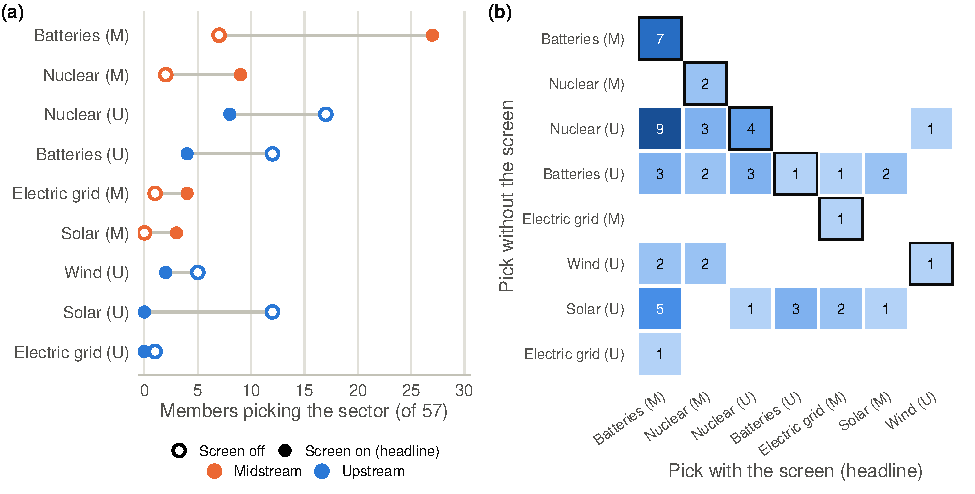
\includegraphics[width=\textwidth]{strategic_screen}
  \caption{Allied picks with and without the endowment screen. Panel (a): number of the 57 members
  whose pick is each sector, with the screen (filled, the headline) and without it (open); colour is
  the stage. Panel (b): transition between the two selections; each tile counts the members whose
  pick without the screen is the row and with it the column; outlined diagonal tiles are unchanged
  picks (16 members). Index values are the same in both selections; the screened selection equals
  \texttt{allied\_strategic.csv}. Source: \texttt{strategic\_index} in \texttt{index\_outputs.rds};
  \texttt{select\_allied\_strategic\_sectors()} with the screen on and off.}
  \label{fig:strategic_screen}
\end{figure}

\paragraph{The security sign and other normative choices.} Reading security as strength, $\ES$ in
place of $1-\ES$, gives an index that agrees only weakly with the headline
(Figure~\ref{fig:strategic_sign}): the median within-member Spearman correlation is 0.36, only 5 of
the 57 picks survive, and picks move to Nuclear Midstream (28), Gas Midstream (10) and Electric Grid
Midstream (7). The sign is the most consequential normative choice: the need reading asks where an
economy should build capability to reduce its exposure, the strength reading where it can build on
capability it has. The other choices keep median within-member correlations of 0.88--0.96 but
change many picks. Of the 57 members, 31 keep their pick without the stage and technology priors, 30
without the policy term, 20 when opportunity and need are ranked within the country, and 34 when the
October 2026 NIPO component is added back (27 of the 50 members with NIPO data); policy from IEA
PAMS alone keeps 45 (34 of the 46 members scored on both components). The headline pick stays in
the variant's top three for 86 to 96 percent of members. Requiring both policy
components removes the 11 members scored on the IEA component alone and leaves the other cells
unchanged. A member's sector ordering is thus robust to these choices, but its single pick is not
(Online Appendix~\ref{oa:strategic}; Section~\ref{sec:robustness}).

\begin{figure}[tbp]
  \centering
  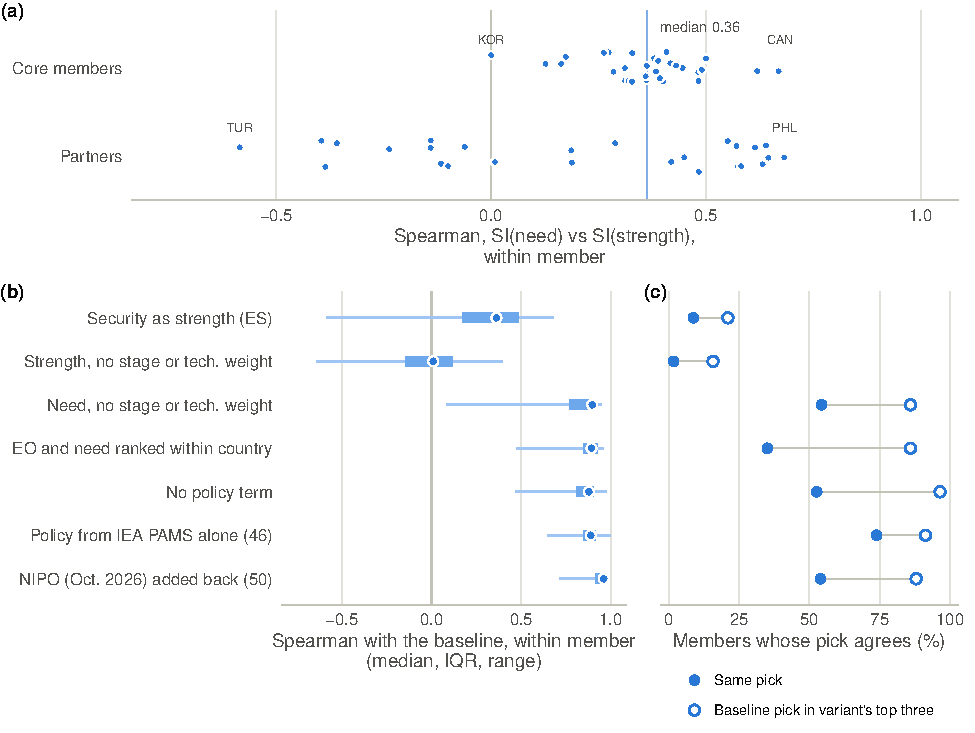
\includegraphics[width=\textwidth]{strategic_sign}
  \caption{Sensitivity of the Strategic Index to its normative choices, coalition members. Panel
  (a): within-member Spearman correlation between the headline index (security as need, $1-\ES$) and
  the index with security as strength ($\ES$), all other terms unchanged; one point per member, by
  tier, median marked. Panel (b): within-member Spearman correlation of each variant with the
  headline (median, interquartile range and range): strength; strength without the stage and
  technology weights; need without those weights; opportunity and need ranked within the country; no
  policy term; policy from the IEA component alone (46 members scored on both); the October 2026 NIPO
  component added back (50 members with NIPO data). Panel (c): share of members whose pick is
  unchanged (filled) and whose headline pick is among the variant's top three (open); the IEA-alone and
  NIPO rows are shares of the 46 and 50 members whose index the variant changes, and over all 57
  members 45 and 34 picks are unchanged (Table~\ref{tab:robustness_picks}). All variants
  keep the endowment screen and the headline cells. Source: \texttt{index\_outputs.rds}; the NIPO
  component of the October 2026 run.}
  \label{fig:strategic_sign}
\end{figure}
